% !TeX root = ./Thesis.tex
\chapter{Cryptography}
\label{Cryptography}

% TODO: Nobody can understand crypto based on this definition. Start with an explanation that foresees what the chapter will contain.
Modern cryptography is based on relatively few mathematical fundamentals. The most dominant  have historically been prime numbers and modular multiplication, but elliptic curve cryptography is increasingly considered to be the most secure method out there to keep things colloquial.

Modular multiplication with large numbers has a useful property that you can exchange encrypted data without the participants knowing each other's private keys, but requiring a computation that is theoretically almost impossible to break. Prime numbers and elliptic curves can be used to create the variables used in modular multiplication, providing the basis for the robustness of the cryptosystem.
% HAH TÄÄ ON IHAN PASKA ATM, get a grip

\section{RSA}

RSA is named after it's discoverers – Rivest, Shamir, Adleman. It is an asymmetric public-key cryptosystem, meaning that it is based on a keypair, in which one is a public and the other is a secret. The public key is used to encrypt, and the secret key is used to decrypt. This means that everyone who has the public key can encrypt data and that encrypted data is practically impossible to decrypt without the secret key. This works due to the fact that it is hard to factor the product of two large prime numbers.

% TODO: Reader thinks what the hell is the next paragraph about, try to open things up a bit before going into factoring competitions, although they play a big part in VDF history

Some institutions also have been publishing these products of two large prime numbers, claiming they have discarded the two prime numbers that were used in the creation. These are published as public puzzles with prizes for correct factorizations as high as 200000 US dollars, but the larger ones can also be used in cryptography to remove a trusted setup. These products are called RSA numbers, of which RSA-1024 and RSA-2048 are widely used. They can be considered relatively safe for production use, since the latest broken RSA number at the time of writing is RSA-250. Still, in practice, the keys could be still stored by the number's creator, requiring trust towards the institutions or individuals who have published them.

% TODO: We might not need this because of Fiat-Shamir, so consider removing this
\section{Diffie-Hellman Key Exchange}

Diffie-Hellman key exchange is a way of generating a shared cryptographic key between two participants. The working principle is that both participants in the exchange do commutative calculations on the input that result in the same output, using prime numbers that result in good cryptographic primitives because of the prime factorization problem, that quarantees the participants' secret keys staying secret and the cryptography hard to break. Diffie-Hellman is most widely used in TLS. TLS is the protocol that is working behind secure http traffic, and most of us probably use Diffie-Hellman key exchange every day. There's also an elliptic curve version of the Diffie-Hellman key exchange, but let's first touch on an example with primes:

\begin{figure}
	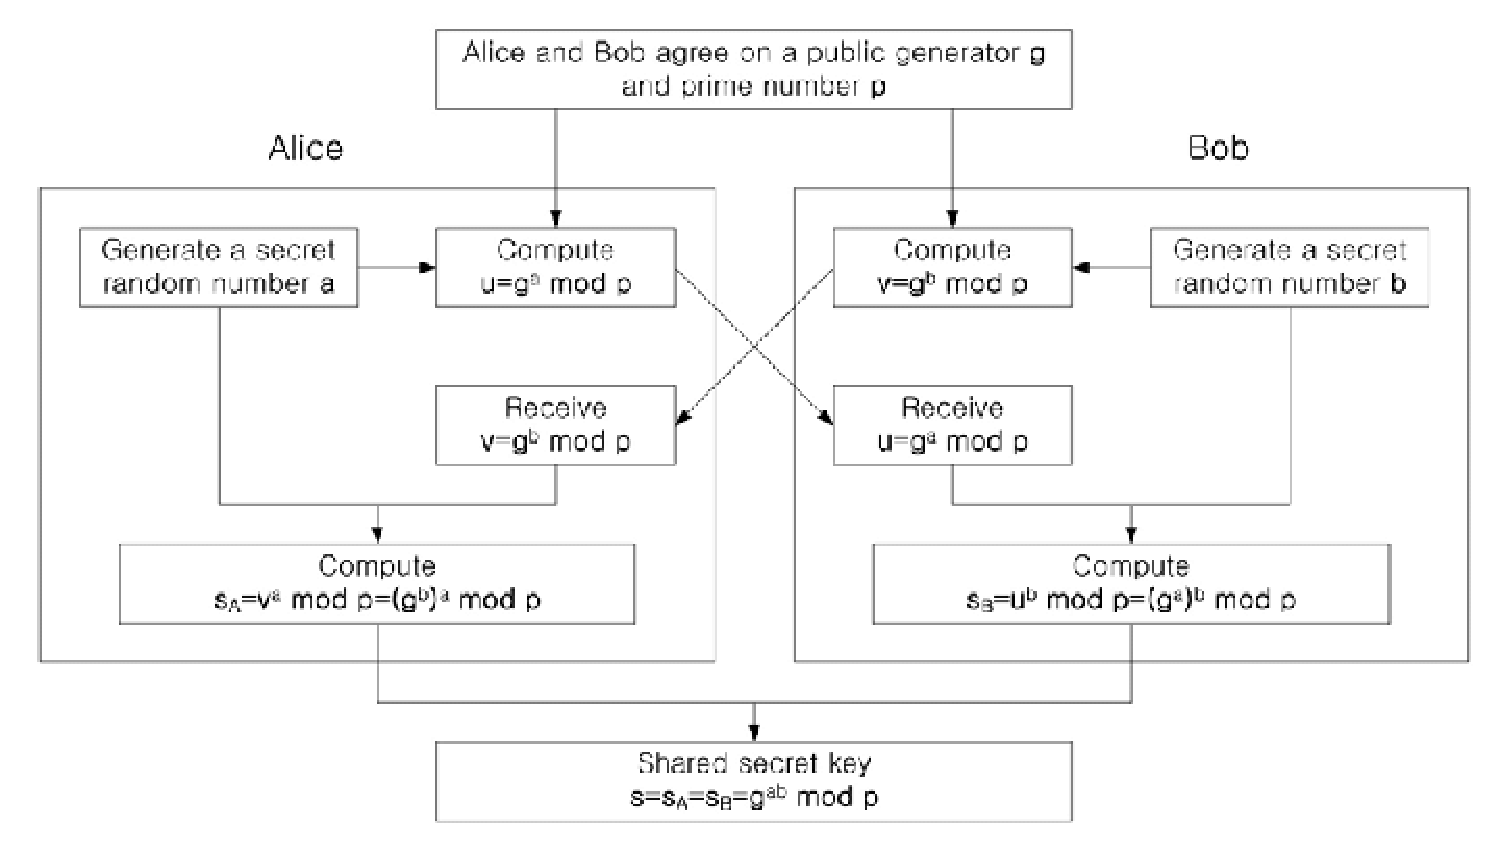
\includegraphics[width=\textwidth]{pictures/diffiehellman.eps}
	\caption{Diffie-Hellman key exchange algorithm\cite{Jeon2014-ag}}
	\label{Diagram, Diffie-Hellman Key Exchange}
\end{figure}

\begin{enumerate}
  \item Alice and Bob agree on a large prime number $p = 941$ and a primitive root of it, $g = 627$.
  \item Alice chooses the secret key $a = 347$ and computes
    \(A = 390 \equiv 627^{347} \ (\bmod 941).\)
  \item Bob chooses the secret key $b = 781$ and computes
    \(B = 691 \equiv 627^{781} \ (\bmod 941).\)
  \item Alice sends bob the number $390$ and Bob sends Alice the number $691$.
  \item Since the operations are commutative, Alice and Bob are now able to compute the number
    \(470 \equiv 627^{347 \times 781} \equiv A^b \equiv B^a \quad (\bmod 941)\)
\end{enumerate}

The number $470$ is their shared secret, which they can use for symmetric encryption. Of course, in the real world, the modulus would have to be a large enough prime, because with $941$ as the modulus the maximum number of tries to break it would be just $940$. 

\section{Elliptic Curve Cryptography}
% TODO: Do I need this? Would make a great filler
						
\chapter{Peer-to-Peer Networking}
\label{Peer-to-Peer Networking}
% TODO: This is not an intro paragraph about P2P. You need to start further back and take a more basic view first. Also, try to describe the upcoming sections more
Although most p2p networks utilize the internet, and thus familiar things like IP addresses to find other peers through the same routers as anyone else, there needs to be a way for nodes to signal their participation in a particular p2p network. Networks that utilize existing infrastructure but build a P2P abstraction on them are called P2P overlay networks. The simplest way to create a P2P network would be to share a single file with anyone who connects to you that has all the IP addresses you've ever connected with. This would be an example of an unstructured P2P network, which could work relatively well in a closed setting, like inside a LAN if there's no support for multicast DNS, or mDNS in short.

\section{Ad Hoc and Zero Configuration Networking}
Multicast DNS was proposed by Apple in 2013~\cite{Cheshire2013-ja} as a way of discovering peers in a local area network in a zero-configuration manner. It is used today for resource sharing, such as sharing printers. Multicast DNS does not work outside local area networks, since it works by associating names with IP addresses like regular DNS does. The problem is that these names are not quaranteed to be unique, and therefore can be spoofed. If there are two clients with the same name, the first one to respond with its IP address to a query wins.~\cite{Pdp2008-tg} The security of zero-configuration and ad hoc networking must relay on cryptographic identities, so that a peer can verify itself with public-key cryptography, that makes the peers on the network practically unique and thus hard to spoof.

% TODO: Seuraavaksi väite, cite!
Zero-configuration networking in an unconstrained, global setting is possible with radios, using either dedicated meshnet radios like GoTenna~\cite{GoTenna} or Helium~\cite{Helium}, or by using the antennas inside mobile devices to form a network. These types of networks are usually called meshnets or ad hoc networks. Basically, Walkie-Talkies are the simplest form of a p2p network. Problems can arise due to geography blocking signals, or when you want to cross large distances with the transmitting capability of a pocket device. Mesh networking has been used most famously in protests worldwide by using a smartphone app called Firechat.~\cite{Milian2014-mt}

Ad hoc mesh networks have a natural metric for latency, signal strength, and thus will not benefit from dynamic routing offered by DHTs as much. They can rely on Bluetooth RSSI\footnote{Received Signal Strength Indication} as a metric, or triangulate distances by cooperating with multiple peers. This type of system is used to locate emergency calls and contact tracing.~\cite{theintercept} Mesh networks, while very much peer to peer and not relying on existing infrastructure like overlay networks, still need routing if one wants to reach peers that are not in the operating range of the communication method used. 

\section{Distributed Hash Tables}
Distributed hash tables are a way of pointing content to peers in a distributed network. In addition to indexing content in content-addressed networks like IPFS~\cite{IPFS}, they can function as routing tables. A hash table is a key-value mapping from a to b. What makes them distributed is the fact that the data stored is meant to be distributed between peers, with not a single peer keeping all the available data in its hash table, but relaying queries for resources it can't reach to other peers on the network. There are multiple versions of DHTs with different methods for prioritizing certain peers, using tree structures, sorting by identifiers, using computational trust et cetera.

Most of the DHT algorithms were invented in the early 2000s, with Kademlia being one of them. DHTs mostly differ just by how distance is defined, and how the neighbors are chosen.~\cite{Cai2015-ra} DHTs have been developed to remove bottlenecks in peer search.
						
\subsection{Kademlia}
Kademlia is a DHT designed by Petar Maymounkov and David Mazières in 2002. It is based on a tree of identifiers which are split across peers on a network. The identifiers are 160 bits, e.g. a SHA-1 hash of some larger data. Kademlia tries to improve upon previous DHT-based routing algorithms by introducing a symmetric XOR metric for distance between node IDs in the key space.~\cite{Petar_Maymounkov2020-sx} These IDs are sorted in a binary search tree, with each node's position determined by the shortest unique prefix of its ID. Kademlia makes sure that any node in the network can locate any other node by its ID by making sure that each node knows at least one of the nodes in each subtree.
						
A single query in Kademlia has been shown in real-world tests to result in an average of 3 network hops, meaning that the query gets relayed through two peers before reaching the requested resource.~\cite{Roos2013-mb} Network hops are a necessary evil in distributed systems, and Kademlia does well in requiring on average a log(n) queries in a network of n nodes. Since the closeness metric is based on a similarity search rather than a measurement, the closest peer is only closest by the identifier, not by network latency.~\cite{Eigenmann2020-zm}
						
The randomness of Kademlia is great at averaging the network hops required to reach a scarce resource. The downside is that it also averages everything else, increasing latency to closest connected peers, and increasing the minimum hops to reach a common resource.

Kademlia protocol has four remote procedure calls, or RPCs in short. These are PING, STORE, FIND\_NODE, and FIND\_VALUE. A Kademlia participant's most important operation is node lookup, which is locating k closest nodes to a given node ID. It is a recursive operation, which starts by picking alpha closest nodes from its closest non-empty bucket, and sending them all FIND\_NODE calls. This is repeated until the initiator has queried and gotten responses from all k closest nodes it has seen.

\subsubsection{Eclipse Attacks}
Although Kademlia is usually used with random hashed identifiers, the distance metric stays the same. By forging identities that are close-by, you can advertise false friends which take over the search space. For example, in a 2019 paper "Eclipsing Ethereum Peers with False Friends" by S. Henningsen, D. Teunis, M. Florian, and B. Scheuermann, they demonstrate that to eclipse a victim in Ethereum p2p network, you need to fill its 8 slots for outbound connections, and fill 17 slots for inbound connections to completely deny service without going through the attacker's nodes.~\cite{Henningsen2019-mf}

% TODO: More stuff here
